\section{Tilstandsmaskin}
\thispagestyle{fancy}

Vi identifiserte tidleg i prosessen eit ynskje om å lage ei tilstandsmaskin som hadde overordna styring over kvar reaktor. 
Sidan ein \gls{SBR}-reaktor er prinsipielt oppbygd av forskjellige sekvensar, virka det logisk å implimentere ei tilstandsmaskin.
Tilstandsmaskina vil ha ansvar for å oppretthalde korrekt tilstand og avansere vidare når gitte kriterier er nådd.

\begin{figure}[htbp]
    \centering
    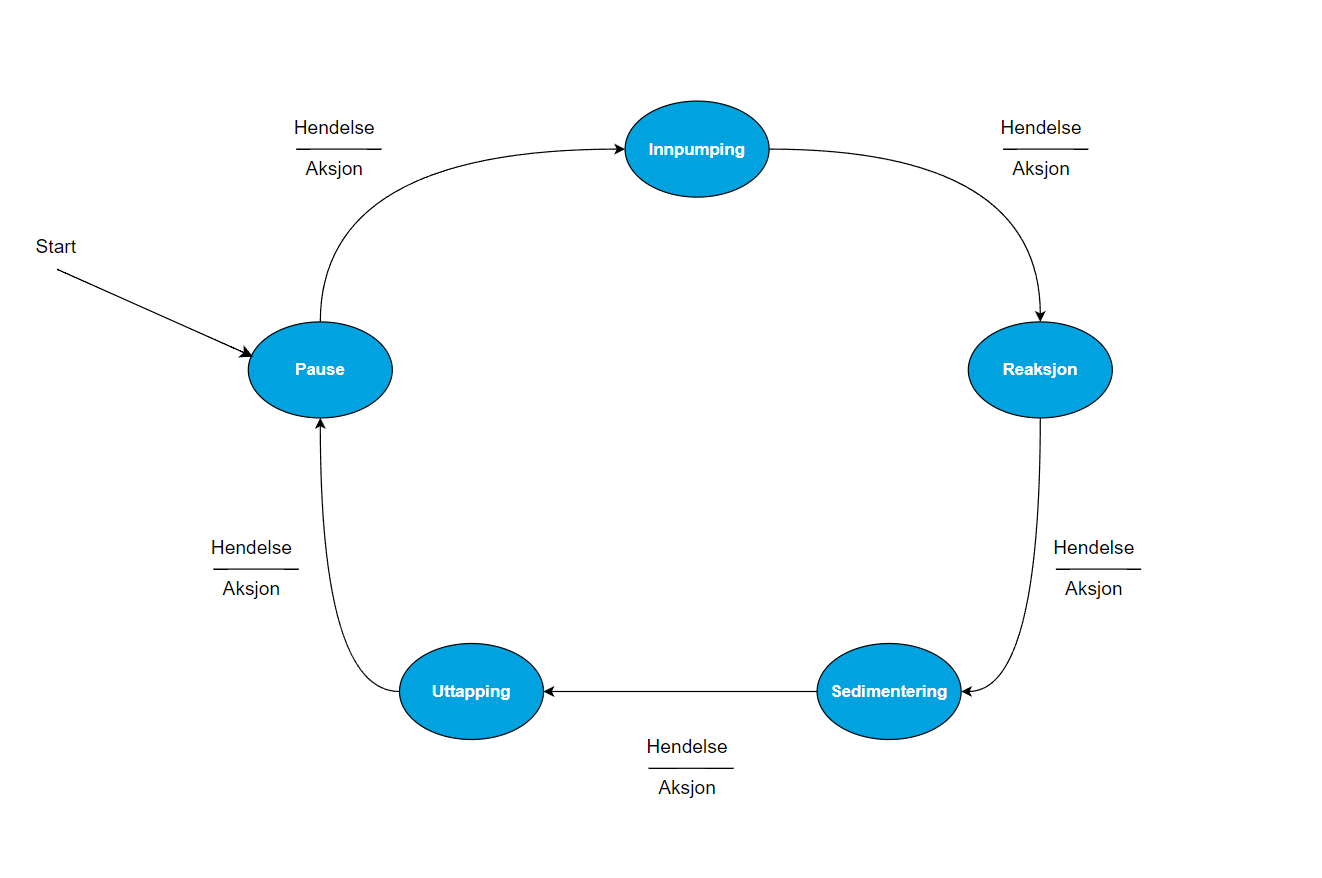
\includegraphics[width=1\textwidth]{Figurar/Tom tilstandsmaskin.png}
    \caption{Tilstandsmaskin prinsipp}\label{fig:Tilstandsmaskin prinsipp}    
\end{figure}

\newpage

